\documentclass[11pt,a4paper]{article}
\usepackage[margin=2.5cm]{geometry}
\usepackage{amsmath,amssymb}
\usepackage{booktabs,array,multirow}
\usepackage{graphicx,float,caption}
\usepackage{xcolor}
\usepackage{listings}
\usepackage{enumitem}
\usepackage{tikz}
\usetikzlibrary{arrows.meta,positioning}
\usepackage[colorlinks=true,linkcolor=teal!50!black,urlcolor=blue!50!black]{hyperref}
\usepackage{microtype}

\setlist{itemsep=3pt,topsep=4pt,parsep=0pt}
\captionsetup{font=small,labelfont=bf}
\setlength{\parindent}{0pt}
\setlength{\parskip}{7pt}
\renewcommand{\arraystretch}{1.18}

\definecolor{cgood}{HTML}{0F766E}
\definecolor{cwarn}{HTML}{C2410C}
\definecolor{cgrey}{HTML}{6B7280}
\newcommand{\tx}[1]{\texttt{\detokenize{#1}}}
\lstset{basicstyle=\ttfamily\footnotesize,breaklines=true,frame=single,rulecolor=\color{black!25},
        backgroundcolor=\color{black!3},columns=fullflexible,keepspaces=true,showstringspaces=false}

\newcommand{\callout}[2]{%
  \begin{center}\begin{tikzpicture}
    \node[draw=#1,fill=#1!7,line width=.8pt,rounded corners=3pt,inner sep=9pt] {\parbox{.9\linewidth}{#2}};
  \end{tikzpicture}\end{center}}

\title{\textbf{Qwen3.5-4B at up to 11{,}000 tokens/s prefill\\ and 200 tokens/s decode on one AMD GPU}\\[4pt]
\large Rotated INT4 on RDNA3: what it is, what it gets you, and how to reproduce it}
\author{}
\date{2 November 2026}

\begin{document}
\maketitle
\vspace{-1.2cm}

%=====================================================================================================================
\section*{The short version}

\callout{cgood}{\textbf{The premise.} Four-bit weights are half the size of eight-bit ones, and the matrix units of AMD's RDNA3 GPUs multiply four-bit integers at
twice the rate of eight-bit ones. llama.cpp does not use them, because plain four-bit models lose accuracy. We make the accuracy loss small enough to use the
hardware: \textbf{rotate} the weights and activations so the outliers disappear, \textbf{quantise} the weights with GPTQ, and \textbf{multiply on the int4 units}.}

On the stock \textbf{Qwen3.5-4B}, on one Radeon RX~7900~XT, against the standard llama.cpp 4-bit format (Q4\_K\_M), measured on the same build in the same session:

\begin{table}[H]
\centering\small
\begin{tabular}{@{}lrrrrrrr@{}}
\toprule
 & \multicolumn{2}{c}{prefill (tokens/s)} & decode & \multicolumn{3}{c}{accuracy vs the BF16 model} & VRAM\\
\cmidrule(lr){2-3}\cmidrule(lr){5-7}
Qwen3.5-4B, 4-bit & pp512 & pp2048 & (tokens/s)$^{\dagger}$ & KLD $\downarrow$ & PPL & top-1 & peak$^{\ddagger}$\\
\midrule
Q4\_K\_M (standard llama.cpp) & 5{,}477 & 5{,}387 & 147.4 & 0.028 & +2.0\% & 91.9\% & 3.62\,GB\\
\textbf{rotated INT4, \tx{quality}} (default) & \textbf{7{,}140} & \textbf{7{,}013} & \textbf{202.2} & \textbf{0.024} & +1.9\% & 92.7\% & 3.36\,GB\\
\textbf{rotated INT4, \tx{fast}} (one setting) & \textbf{11{,}012} & \textbf{10{,}624} & \textbf{202.0} & 0.097 & +8.7\% & 86.1\% & 3.36\,GB\\
\bottomrule
\end{tabular}\\[2pt]
\parbox{.97\linewidth}{\scriptsize $^{\dagger}$Decode after a 128-token context; from an empty context every row is 1.4--2.2 tokens/s lower and the ratios are the same to within 0.01.
$^{\ddagger}$Peak GPU memory during prefill plus decode, measured for \tx{quality}; \tx{fast} uses the same weights.}
\end{table}

\begin{itemize}
\item \textbf{\tx{quality}} is the same accuracy as Q4\_K\_M (perplexity +1.9\% against +2.0\%; slightly lower KLD and higher top-1) at \textbf{1.3$\times$ the prefill speed and
1.4$\times$ the decode speed}, in 7\% less memory.
\item \textbf{\tx{fast}} is one environment variable away: \textbf{2.0$\times$ the prefill speed} of Q4\_K\_M, same decode speed, at a measured accuracy cost
(perplexity +8.7\%, KLD 0.097).
\item \textbf{It is not specific to one model.} The same recipe on Ossicle-4B, a fine-tune of the same backbone with an audio encoder, gives the same speed and the same
accuracy pattern (Section~\ref{sec:ossicle}).
\end{itemize}

\paragraph{How to read the numbers.} \emph{Prefill} is reading the prompt (pp512 = a 512-token prompt); \emph{decode} is writing the answer one token at a time.
\emph{KLD} is how far the model's output probabilities have moved from the original BF16 model (lower is better); \emph{PPL} is the same comparison as a perplexity change on
WikiText-2; \emph{top-1} is how often both models pick the same next token. Accuracy: 24 chunks of WikiText-2 test (about 12{,}000 tokens), context 512, each model compared with
its own BF16 original; the standard error of a KLD is about $\pm0.001$--$0.002$ for the first two rows and $\pm0.003$ for \tx{fast}. Speed: median of eight \tx{llama-bench} runs
after dropping the first. Q4\_K\_M was built from the same BF16 file with an importance matrix from WikiText-2 train, like a user would.

%=====================================================================================================================
\section{The idea in three steps}

\begin{figure}[H]
\centering
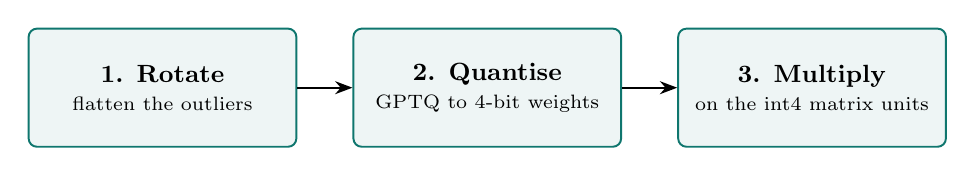
\begin{tikzpicture}[node distance=7mm,box/.style={draw=cgood,fill=cgood!7,rounded corners=3pt,minimum height=15mm,minimum width=34mm,align=center,font=\small,line width=.7pt},
  arr/.style={-{Stealth[length=2.2mm]},line width=.7pt}]
\node[box] (a) {\textbf{1. Rotate}\\[-1pt]\scriptsize flatten the outliers};
\node[box,right=of a] (b) {\textbf{2. Quantise}\\[-1pt]\scriptsize GPTQ to 4-bit weights};
\node[box,right=of b] (c) {\textbf{3. Multiply}\\[-1pt]\scriptsize on the int4 matrix units};
\draw[arr] (a)--(b); \draw[arr] (b)--(c);
\end{tikzpicture}
\end{figure}

\textbf{1.\ Rotate.} A language model's activations contain a few channels with huge values. Rounding to four bits ruins them, which is why naive 4-bit models are bad.
Multiplying by a Hadamard-style rotation (an orthogonal matrix) before rounding spreads each outlier evenly over 256 values. Because the rotation is orthogonal, rotating the weights
\emph{offline} and the activations \emph{at run time} gives exactly the original result before rounding, so nothing is lost by doing it.

\textbf{2.\ Quantise.} The rotated weights are rounded to symmetric 4-bit integers with GPTQ (error-compensated rounding using 128 calibration sequences of WikiText-2 text),
with one scale per 32 weights. The result is stored as a normal-looking GGUF file of the same size as Q4\_0 (2.55\,GB for this model including a Q6\_K output head).

\textbf{3.\ Multiply on int4 units.} RDNA3 has matrix instructions for 4-bit integers at twice the int8 rate. The weights stay 4-bit; the activations are 8-bit (the
default, \tx{quality}: two 4-bit passes) or 4-bit (\tx{fast}: a single pass, twice as fast and less accurate). Decode always uses 8-bit activations.

\begin{center}\small
\begin{tabular}{@{}llll@{}}
\toprule
preset & activations & how to select & what it is for\\
\midrule
\tx{quality} & 8-bit (two int4 passes) & default & Q4\_K\_M-level accuracy, faster\\
\tx{fast} & 4-bit (one int4 pass) & \tx{GGML_INT4_PREFILL=fast} & maximum prefill speed, accuracy cost\\
\bottomrule
\end{tabular}
\end{center}

%=====================================================================================================================
\section{Result: stock Qwen3.5-4B}
\label{sec:stock}



Figure~\ref{fig:stock} in three sentences. The default preset keeps accuracy where Q4\_K\_M has it and is 30\% faster at reading the prompt and 37\% faster at writing.
The \tx{fast} preset doubles the prompt speed and pays for it in accuracy: its KLD is 3.5$\times$ Q4\_K\_M's. Decode speed is the same in both presets because decode does not
use the 4-bit-activation path.

\paragraph{What this does not claim.} The \tx{quality} advantage in \emph{accuracy} over Q4\_K\_M is small: perplexity is equal within noise, and the KLD difference
(0.024 against 0.028) is only a little larger than the error bars. The claim is ``same accuracy, clearly faster'', not ``more accurate''. The \tx{fast} preset is not free.

\begin{figure}[H]
\centering\includegraphics[width=\linewidth]{fig/sum_stock.pdf}
\caption{\label{fig:stock}Stock Qwen3.5-4B on one RX~7900~XT. The multipliers are against Q4\_K\_M. Prefill is pp512; decode is after a 128-token context.}
\end{figure}

%=====================================================================================================================
\section{It is not Ossicle-specific}
\label{sec:ossicle}

This work started on Ossicle-4B, an audio--language model whose language backbone is Qwen3.5-4B. The obvious objection is that the recipe only works for that model. So we ran
the \emph{identical pipeline} on the untouched Qwen3.5-4B checkpoint from Hugging Face and measured both models the same way, on the same build:

\begin{table}[H]
\centering\small
\begin{tabular}{@{}llrrrrrr@{}}
\toprule
model & format & pp512 & pp2048 & decode & KLD & PPL & top-1\\
\midrule
\multirow{3}{*}{\begin{tabular}[c]{@{}l@{}}Qwen3.5-4B\\ (stock)\end{tabular}}
 & Q4\_K\_M & 5{,}477 & 5{,}387 & 147.4 & 0.028 & +2.0\% & 91.9\%\\
 & rotated INT4 \tx{quality} & 7{,}140 & 7{,}013 & 202.2 & 0.024 & +1.9\% & 92.7\%\\
 & rotated INT4 \tx{fast} & 11{,}012 & 10{,}624 & 202.0 & 0.097 & +8.7\% & 86.1\%\\
\midrule
\multirow{3}{*}{\begin{tabular}[c]{@{}l@{}}Ossicle-4B\\ (fine-tune)\end{tabular}}
 & Q4\_K\_M & 5{,}461 & 5{,}356 & 147.2 & 0.031 & +3.5\% & 91.2\%\\
 & rotated INT4 \tx{quality} & 7{,}094 & 6{,}992 & 202.0 & 0.025 & +2.0\% & 92.3\%\\
 & rotated INT4 \tx{fast} & 10{,}934 & 10{,}606 & 202.3 & 0.101 & +9.1\% & 85.0\%\\
\bottomrule
\end{tabular}
\caption{Both models, one pipeline, one build. Accuracy is each model against its own BF16 original. Same units as the first table.}
\end{table}

\begin{figure}[H]
\centering\includegraphics[width=.64\linewidth]{fig/sum_plane.pdf}
\caption{Speed against accuracy for both models. Circles: stock Qwen3.5-4B. Squares: Ossicle-4B. The two models sit on top of each other.}
\end{figure}

The two models behave the same: speed within 1\% (the architecture is identical, so the kernels do the same work), the ordering \tx{quality} better than Q4\_K\_M and
\tx{fast} much faster but less accurate in both, and \tx{fast}'s KLD at 3.2--3.5$\times$ Q4\_K\_M's in both. Nothing in the method is specific to Ossicle: the stock model goes through the same scripts (Section~\ref{sec:repro}); the only change was teaching the GPTQ script to read the
original checkpoint's tensor names. Ossicle's extra parts (audio encoder, fine-tuned weights) are not involved in these measurements.

\paragraph{What this does not show.} Both models are 4~billion-parameter models of one architecture (Qwen3.5: gated-delta-net layers alternating with full attention). We have
\emph{not} measured other model families or sizes. That is the next test, not something this document claims.

%=====================================================================================================================
\section{Why it is faster}

\paragraph{Prefill: the int4 units are the fast ones.} Prefill is compute-bound. The standard llama.cpp 4-bit path unpacks 4-bit weights to 8-bit and uses the int8 matrix
units, which reach about 36--40 TOPS on this card in our tests. Ours feeds the int4 units directly and reaches about 134 int4-TOPS (74\% of the hardware's int4 peak): in \tx{quality} mode that is the
same work as 67 int8-TOPS, in \tx{fast} mode twice that. We also rewrote the linear-attention and full-attention kernels on the matrix units and fused many small operations into
their neighbours.

\paragraph{Decode: stop launching so many kernels.} Decode is memory-bound: each token reads the whole 2.5\,GB of weights, which at this card's 750\,GB/s takes 3.4\,ms, a ceiling of
about 297 tokens/s. The first version spent over a third of each token idle, launching 847 tiny GPU kernels. Fusing them into 236 raised decode from 138 to 200 tokens/s, now 67\% of the ceiling.
What remains is about 1\,ms per token of gaps between kernel launches.

\begin{figure}[H]
\centering\includegraphics[width=.78\linewidth]{fig/sum_decode.pdf}
\caption{Decode speed against kernel launches per token, through the work (readings from different sessions; decode from an empty context).}
\end{figure}

%=====================================================================================================================
\section{Why the accuracy holds}

\begin{itemize}
\item \textbf{Rotation makes four bits usable.} Without it, the outlier channels dominate the rounding error. With it, each 256-value block is close to Gaussian, which is what
low-bit rounding handles well.
\item \textbf{The activations decide the accuracy, not the weights.} Four-bit weights with 8-bit activations (\tx{quality}) land at KLD 0.024; changing only the activations to
4-bit (\tx{fast}) takes it to 0.097. Eight bits of activation are enough; four are not, which is why \tx{fast} costs accuracy and \tx{quality} does not.
\item \textbf{GPTQ and small groups.} In our simulations on Ossicle-4B, GPTQ was worth about 0.03 KLD over plain rounding, and one scale per 32 weights beat one per 64 or 128 by
0.01--0.02 KLD. The technical report has the full ablation.
\end{itemize}

%=====================================================================================================================
\section{Reproduce it on stock Qwen3.5-4B}
\label{sec:repro}

You need an RDNA3 GPU (we used an RX~7900~XT, ROCm~10.1.0), about 15\,GB of system RAM for the GPTQ step, and about 20\,GB of disk, and WikiText-2 (\tx{wiki.train.raw}, \tx{wiki.test.raw}). The GPTQ step itself takes about four minutes.

\begin{lstlisting}[language=bash]
# 0. llama.cpp fork with the INT4 path (branch "ossicle"), built for RDNA3
cmake -S . -B build -DGGML_HIP=ON -DAMDGPU_TARGETS=gfx1100 -DCMAKE_BUILD_TYPE=Release && cmake --build build -j

# 1. the unmodified model from Hugging Face -> BF16 GGUF
huggingface-cli download Qwen/Qwen3.5-4B --local-dir qwen35-4b
python convert_hf_to_gguf.py qwen35-4b --outtype bf16 --no-mtp --outfile qwen35-4b-bf16.gguf

# 2. GPTQ on the rotated weights (about 4 minutes, about 15 GB RAM; calibration text = WikiText-2 train)
python scripts/gptq_rotate.py --src qwen35-4b --out gptq_g32.safetensors --group 32 --calib 128

# 3. write the GGUF (checks every tensor against the BF16 weights; Q6_K output head)
python scripts/rotate_quantize.py qwen35-4b-bf16.gguf qwen35-4b-rotq4-gptq.gguf --blocks gptq_g32.safetensors --embd q6_k

# 4. run it
llama-server -m qwen35-4b-rotq4-gptq.gguf -ngl 99                           # quality (default)
GGML_INT4_PREFILL=fast llama-server -m qwen35-4b-rotq4-gptq.gguf -ngl 99    # fast

# 5. check the numbers in this document
llama-bench -m qwen35-4b-rotq4-gptq.gguf -ngl 99 -p 512,2048 -n 128 -d 0,128 -r 9
llama-perplexity -m qwen35-4b-bf16.gguf -f wiki.test.raw -c 512 -ngl 99 --chunks 24 --kl-divergence-base base.bin   # saves the BF16 reference
llama-perplexity -m qwen35-4b-rotq4-gptq.gguf -f wiki.test.raw -c 512 -ngl 99 --chunks 24 --kl-divergence-base base.bin --kl-divergence
\end{lstlisting}

The Q4\_K\_M baseline in this document was made from the same BF16 file with \tx{llama-imatrix} (WikiText-2 train, 250 chunks of 1024 tokens)
and \tx{llama-quantize} with that importance matrix, and measured with the same commands.

%=====================================================================================================================
\section{Limits}

\begin{itemize}
\item \textbf{RDNA3 only.} The speed comes from RDNA3's int4 matrix instructions (RX~7000 series; we tested one RX~7900~XT). Other GPUs would need their own kernels.
\item \textbf{Not an ordinary GGUF.} The files look like Q4\_0 but hold rotated codes; any build other than this branch decodes them as garbage. The GGUF carries a key that the branch
detects.
\item \textbf{One architecture, one size.} Two models, both 4B Qwen3.5. Other families and sizes are untested.
\item \textbf{\tx{fast} is a trade.} 2$\times$ prefill for KLD 0.097 against 0.024; choose per use case. We do not call it equivalent to \tx{quality}.
\item \textbf{Text calibration.} GPTQ used WikiText-2 text only; the accuracy numbers are text numbers.
\item \textbf{Measurement noise.} A decode figure moves by about $\pm1.5$ tokens/s with GPU temperature, which is why the comparisons are against Q4\_K\_M measured in the
same session. The first prefill sample of a run is slow, so the table uses the median after dropping it.
\item \textbf{Untested:} multi-GPU, loading and unloading a model in one process, long contexts for the new attention path beyond the figures in the technical report.
\end{itemize}

\section*{Where everything is}
Code: the \tx{ossicle} branch of the llama.cpp fork (\tx{SILVERTHRONE32/llama.cpp-ossicle}); files: \tx{SILVERTHRONE/Ossicle-4B-GGUF}, with the stock-model file at
\tx{rdna3/qwen35-4b-rotq4-gptq.gguf}. Licence: Apache~2.0. Every experiment, including the failed ones, is in the full technical report
(\emph{Q4-quality INT4 inference for Ossicle-4B on RDNA3}), which this document summarises.

\end{document}
